%        1         2         3         4         5         6         7         8

\documentclass[letterpaper,10pt,conference]{ieeeconf}



\IEEEoverridecommandlockouts

\overrideIEEEmargins



\usepackage[caption=false,font=footnotesize]{subfig}

\usepackage{graphicx}

\usepackage{booktabs}

\usepackage{array}

\usepackage{algorithm}

\usepackage{algpseudocode}

\usepackage{amsmath}

\usepackage{amssymb}

\usepackage{cite}

\usepackage{xurl}



\makeatletter

\let\NAT@parse\undefined

\makeatother

\usepackage[
    colorlinks=true,
    citecolor=blue,
    linkcolor=blue,
    urlcolor=blue
]{hyperref}



\title{\LARGE \bf
A Structured LLM-Assisted Decision Pipeline for Unsignalised Intersection Control in SUMO
}



\author{Cheng Peng}



\begin{document}
\begin{titlepage}
    \begin{center}
        \vspace*{1cm}
        {\huge A Structured LLM-Assisted Decision Pipeline for Unsignalised Intersection Control in SUMO}
        \vspace{0.5cm}

        {\large By}

        \vspace{0.5cm}
        \textbf{PENG, CHENG}
        \vspace{1.5cm}

        {\huge\textbf{MSc Robotics Dissertation}}

        \vspace{10mm}
        
\includegraphics[scale=0.6]{logos/bristolcrest_colour.pdf}
        \hspace{5mm}
        
\includegraphics[scale=0.35]{logos/UWE_insignia.png}

        \vspace{10mm}
        {\large School of Engineering Mathematics and Technology\\
        \textsc{University of Bristol}}\par

        \vspace{0.2cm}

        \&\par

        \vspace{0.2cm}

        {\large School of Engineering\\
        \textsc{University of the West of England}}\par

        \vspace{0.8cm}
        \begin{minipage}{10cm}
        \centering
        A MSc dissertation submitted to the University of Bristol and the University of the West of England in accordance with the requirements of the degree of \textsc{Master of Science in Robotics} in the Faculty of Engineering.
        \end{minipage}\par
        \vspace{0.8cm}
        \today
    \end{center}

    \vspace{1cm}
    {\large{Declaration of own work}}

    I declare that the work in this MSc dissertation was carried out in accordance with the requirements of  the University\'s Regulations and Code of Practice for Research Degree Programmes and that it  has not been submitted for any other academic award. Except where indicated by specific  reference in the text, the work is the candidate\'s own work. Work done in collaboration with, or with the assistance of, others, is indicated as such. Any views expressed in the dissertation are those of the author.

    \begin{flushright}
    Name and Date
    \end{flushright}

    \vspace{1cm}
    {\large{Ethics statement}}

    \textit{To fill in according to the Dissertation Handbook Section 3.2.}

    \begin{flushright}
    Name and Date
    \end{flushright}
\end{titlepage}

\maketitle
\thispagestyle{empty}
\pagestyle{empty}

\begin{abstract}

Large language models (LLMs) offer a potential mechanism for context-aware decision making in autonomous traffic systems, but evaluating their contribution is difficult when they operate within pipelines that also contain deterministic fallback, post-processing, and safety mechanisms. This work develops and evaluates a modular LLM-assisted control framework for cooperative decision making at an unsignalised intersection using the SUMO microscopic traffic simulator. Four controller configurations are considered: a standalone rule-based baseline, Raw LLM, Hybrid, and Hybrid with deterministic safety verification. The formal evaluation comprises 24 valid runs across four- and eight-vehicle scenarios and three random seeds. Across the retained experiments, the three LLM-assisted pipelines achieved substantially lower operational waiting and higher mean speed than the rule-based baseline while maintaining 100\% completion and zero recorded collisions. However, live-provider success during the formal experiment was low, meaning that these traffic improvements cannot be attributed independently to successful LLM reasoning. A subsequent post-hoc diagnostic using a reliable Gemini configuration achieved 53/53 successful provider requests with no fallback, but produced the same traffic outcome as deterministic fallback-only control and matched its decisions on all 132 comparable vehicle-level records. These findings demonstrate a distinction between pipeline-level performance and model-level attribution. The principal contribution of this work is therefore an attribution-aware evaluation framework that combines traffic performance, provider reliability, decision provenance, deterministic fallback analysis, and decision-level comparison to expose both the capabilities and identifiability limitations of LLM-assisted traffic control.

\end{abstract}



\section{Introduction}



Unsignalised intersections are a compact but challenging example of cooperative decision making in autonomous transportation. Multiple vehicles may approach a shared conflict region simultaneously, and each vehicle must determine whether to proceed, wait, or yield while accounting for the intentions and movements of others. A controller that is overly conservative can maintain conflict avoidance at the cost of unnecessary waiting and low traffic efficiency, whereas an overly permissive controller can increase the risk of incompatible movements. Effective intersection management therefore requires a balance between efficiency, coordination, and safety.



Traditional approaches to autonomous intersection management generally rely on predefined traffic rules, reservation mechanisms, optimisation, or explicit cooperative policies \cite{Dresner2008,Safarov2022,Zhao2025}. These approaches provide deterministic and interpretable behaviour, but their decisions are typically constrained by assumptions encoded during system design. As traffic interactions become more context dependent, this motivates investigation into decision mechanisms that can reason over structured descriptions of the current traffic state rather than relying exclusively on a fixed set of handcrafted rules.



Large language models (LLMs) provide one possible mechanism for such context-sensitive reasoning. Recent work has demonstrated the use of language models for planning, embodied reasoning, and decision support in autonomous systems \cite{Huang2022,Driess2023,Wen2023,Jin2023,Cui2024,Yang2024,Hou2025,Yang2024,Li2024}. In principle, an LLM can receive a structured representation of an intersection state and produce high-level actions for multiple vehicles. This makes LLMs attractive as a flexible reasoning component within a modular traffic-control pipeline.



However, integrating an LLM into a safety-relevant control system introduces an important evaluation problem. A practical LLM-assisted controller cannot normally rely on the model alone. Provider requests may fail or experience high latency, generated responses may violate the required output format, and model decisions may require deterministic validation before execution. Consequently, an operational pipeline may also contain parsing, fallback policies, cooperative post-processing, and safety verification. These components improve robustness, but they make the source of observed performance difficult to identify. If an LLM-assisted pipeline outperforms a conventional baseline, the improvement may originate from successful model reasoning, deterministic fallback behaviour, downstream processing, or a combination of these mechanisms.



This distinction between \emph{pipeline-level performance} and \emph{model-level attribution} motivates the present study. Rather than asking only whether an LLM can be connected to a traffic simulator, this work investigates whether an LLM-assisted cooperative control pipeline can improve simulated intersection performance and whether any observed improvement can be attributed to the live language model itself. This requires evaluation at both the traffic level and the internal decision-pipeline level. Traffic metrics describe the behaviour of the complete controller, whereas provider diagnostics, fallback records, and decision provenance are required to determine which component actually produced the executed actions.



To investigate this problem, a modular control framework is implemented using the SUMO microscopic traffic simulator. The framework separates state representation, LLM interaction, structured-output parsing, deterministic fallback, cooperative post-processing, safety verification, and final action execution. Three LLM-assisted configurations are compared with a standalone rule-based baseline: Raw LLM, Hybrid, and Hybrid with Safety. The formal experiment evaluates all four controllers under four-vehicle (4V) and eight-vehicle (8V) scenarios using three random seeds, giving 24 retained runs. Traffic-level metrics include completion, operational waiting, mean speed, throughput, and collisions, while pipeline-level diagnostics record provider success, parser success, fallback use, latency, intervention, and decision provenance.



The study addresses the following research questions:



\begin{itemize}

    \item \textbf{RQ1:} How does the Raw LLM pipeline compare with a standalone rule-based controller in traffic efficiency and completion?

    \item \textbf{RQ2:} Does cooperative post-processing provide an observable benefit beyond Raw LLM control?

    \item \textbf{RQ3:} Does deterministic safety verification provide an observable benefit beyond the Hybrid controller?

    \item \textbf{RQ4:} How do the evaluated controller pipelines behave when the tested traffic scale increases from 4V to 8V?

\end{itemize}



The formal results show a clear pipeline-level difference: the three LLM-assisted configurations achieve substantially lower operational waiting and higher mean speed than the selected rule-based baseline while retaining full completion and zero recorded collisions in the evaluated scenarios. However, provider diagnostics reveal that successful live-model responses are rare in the retained formal runs. The formal experiment therefore establishes a performance difference between complete controller pipelines, but it does not establish that successful LLM reasoning independently caused that difference.



To examine this attribution problem directly, a supplementary post-hoc diagnostic was conducted using a reliable Gemini configuration. Once provider failure was removed as the dominant confound, Gemini successfully completed all 53 logical requests without fallback. Nevertheless, its executed traffic outcome remained identical to a deterministic fallback-only ablation, and its decisions agreed with the fallback on all 132 comparable vehicle-level records. A further high-discrimination subset also failed to produce behavioural divergence. These observations indicate that provider reliability and behavioural identifiability are separate experimental issues: reliable model execution is necessary for evaluating an LLM, but it is not sufficient to demonstrate an independent model contribution.



The contributions of this work are therefore threefold. First, it develops a modular and reproducible LLM-assisted intersection-control pipeline in which model interaction, deterministic recovery, cooperative processing, safety verification, and execution can be examined separately. Second, it provides a controlled comparison of four controller configurations across two traffic scales while preserving traffic-level and provider-level evidence. Third, it demonstrates an attribution-aware evaluation methodology combining provider diagnostics, request provenance, fallback ablation, and decision-level agreement analysis. The resulting evidence supports a pipeline-level traffic-performance contribution while also identifying a limitation of the current experimental design: substantial semantic overlap between the LLM policy and deterministic fallback restricts causal identification of an independent LLM effect.



\section{Related Work}



\subsection{Autonomous Intersection and Cooperative Control}



Autonomous intersection management has long been studied as a coordination problem in which multiple vehicles compete for access to a shared conflict region. Dresner and Stone \cite{Dresner2008} demonstrated that intersection control can be formulated through explicit coordination between autonomous vehicles and an intersection-management mechanism, providing an alternative to conventional fixed traffic signals. Subsequent research has explored reservation-based, optimisation-based, and cooperative approaches to improve traffic efficiency while maintaining safe separation between conflicting movements \cite{Safarov2022}. These studies establish an important principle for the present work: intersection performance depends not only on individual vehicle behaviour but also on how access to the shared region is coordinated.



Cooperative control extends this idea by considering the interaction between multiple vehicles rather than treating each vehicle independently. Zhao et al. \cite{Zhao2025} show how cooperative decision mechanisms can improve the management of interacting vehicles by incorporating information about other participants and their potential conflicts. Such approaches are particularly relevant at unsignalised intersections, where the absence of fixed signal phases makes the ordering and compatibility of vehicle movements central to both efficiency and safety.



Despite their advantages, conventional cooperative methods normally encode their decision logic explicitly through rules, optimisation objectives, reservations, or learned policies. This provides predictability and facilitates verification, but behaviour remains bounded by the representations and decision mechanisms selected during system design. A fixed rule set may therefore become conservative when several vehicles interact simultaneously, while a more complex optimisation-based controller may require additional modelling assumptions and computational machinery. These limitations motivate investigation of reasoning components that can interpret a structured traffic state and select among a constrained set of high-level actions.



The present study does not attempt to replace established intersection-management methods with unconstrained language generation. Instead, the LLM is embedded within a structured control pipeline and operates over a small discrete action space. This preserves deterministic execution while allowing the model to participate in high-level coordination decisions. The rule-based controller remains an independent baseline against which the performance of the complete LLM-assisted pipelines can be compared.



\subsection{LLM Planning and Autonomous Driving}



The emergence of large language models as planning and reasoning components has motivated their application beyond conventional text generation. Huang et al. \cite{Huang2022} demonstrated that language models can use semantic knowledge to support high-level planning, while Driess et al. \cite{Driess2023} showed how large multimodal models can connect language, perception, and embodied decision making. These studies suggest that pretrained models can provide flexible reasoning over structured or semantically meaningful representations without requiring every possible situation to be encoded as an explicit handcrafted rule.



This capability has also attracted interest in autonomous-driving research. DiLu \cite{Wen2023} investigates the use of large language models as knowledge-driven decision agents for autonomous driving, while SurrealDriver \cite{Jin2023} explores LLM-based driving agents and the use of human-like driving knowledge. Other studies examine language-model reasoning, planning, and decision support in driving-related settings \cite{Cui2024,Yang2024,Hou2025}. Recent surveys further indicate a broader trend toward incorporating foundation models and LLMs into autonomous-driving architectures as reasoning or decision-support components \cite{Yang2024,Li2024}.



A recurring design pattern in this literature is the separation between high-level reasoning and low-level execution. An LLM may interpret a scene, reason about interactions, or propose an action, while deterministic software remains responsible for validating and executing the resulting command. This separation is appropriate for traffic control because free-form model output cannot be applied directly to vehicle motion. The model output must first be converted into a constrained action representation that can be interpreted consistently by the simulator or vehicle controller.



The framework developed in this work follows this modular principle. Rather than asking the LLM to generate trajectories or continuous control signals, the model receives a structured description of the intersection state and assigns one of three high-level actions: \texttt{PROCEED}, \texttt{WAIT}, or \texttt{FREE}. A parser validates the structured response before downstream deterministic stages process the decision. This design reduces the interface between probabilistic reasoning and deterministic control to a small and auditable action space.



However, demonstrating that an LLM can be inserted into such a pipeline does not establish that it provides a useful independent contribution. A system can continue to operate when the model fails if deterministic fallback or downstream control logic supplies the executed action. Consequently, traffic-level success alone may overstate the evidence for model-level reasoning.



\subsection{Reliability, Hybrid Control, and the Attribution Problem}



Reliability is particularly important when LLMs are used within operational decision pipelines. Model outputs may be affected by provider availability, latency, output-format violations, or inconsistent reasoning. More broadly, evaluations of language-model agents have shown that plausible model behaviour should not automatically be interpreted as reliable or grounded decision making \cite{Xie2025}. For a traffic-control application, these concerns mean that model quality must be considered together with the behaviour of the surrounding software system.



One practical response is to use a hybrid architecture. A live model can provide a candidate decision when a valid response is available, while deterministic mechanisms handle request failure, invalid output, conflict resolution, or safety constraints. Such an architecture can be more operationally robust than direct model control because the simulator does not depend entirely on successful provider responses. However, robustness introduces an evaluation ambiguity. If deterministic fallback frequently replaces unavailable model output, strong traffic performance may primarily reflect the fallback policy. Similarly, if cooperative post-processing or a safety verifier modifies model decisions before execution, the final traffic outcome may differ from the behaviour proposed by the model.



This creates a distinction between \emph{traceability} and \emph{causal identifiability}. Traceability concerns whether an experiment records the sequence of events inside the controller, such as whether a provider request was attempted, whether parsing succeeded, whether fallback was activated, and which final action was executed. Causal identifiability concerns the harder question of whether the observed outcome would have changed in the absence of a particular component. A highly instrumented system may therefore be traceable without providing sufficient experimental variation to isolate the independent effect of its LLM.



This distinction motivates the evaluation strategy used in this work. Traffic metrics are used to compare the complete controller pipelines, while provider diagnostics and provenance records identify how those outcomes were produced. In addition, deterministic fallback ablation and decision-level comparison are used as post-hoc attribution tools when formal traffic results alone cannot distinguish live-model behaviour from deterministic substitution. This is especially important because the fallback policy and the LLM prompt may encode overlapping traffic-control semantics.



The resulting research gap is therefore narrower than the general question of whether LLMs can participate in autonomous-driving systems. Existing studies provide substantial motivation for using language models in planning and driving-related decision pipelines \cite{Wen2023,Jin2023,Cui2024,Yang2024,Li2024}, while autonomous-intersection research establishes the importance of cooperative access management \cite{Dresner2008,Safarov2022,Zhao2025}. What remains less explicit is how to evaluate the independent contribution of an LLM when the operational controller also contains deterministic mechanisms capable of producing similar decisions. The present work addresses this gap through an attribution-aware experimental design that evaluates both the external traffic behaviour of the complete pipeline and the internal provenance of the decisions that produced it.



\section{Methodology}



\subsection{System Architecture}



The proposed framework implements intersection control as a modular decision pipeline connecting the SUMO microscopic traffic simulator \cite{AlvarezLopez2018} to either deterministic or LLM-assisted decision logic. At each decision point, the controller obtains the current simulation state, constructs a structured representation of the relevant vehicles, selects or requests high-level actions, validates the resulting decisions, and converts them into commands that can be executed by the simulator. Figure~\ref{fig:architecture} summarises this architecture.



The pipeline is deliberately separated into distinct stages rather than treating the LLM as an end-to-end vehicle controller. The principal stages are: (1) traffic-state extraction from SUMO, (2) construction of the decision context, (3) live-provider inference for LLM-enabled configurations, (4) structured-output parsing and validation, (5) deterministic fallback when a usable model response is unavailable, (6) optional cooperative post-processing, (7) optional deterministic safety verification, and (8) execution and diagnostic recording. This decomposition allows the same simulation environment and action interface to be retained while individual decision mechanisms are changed between controller configurations.



The four evaluated controllers use different subsets of this architecture. The \emph{Rule-Based} controller is a standalone deterministic baseline and does not depend on a live language model. \emph{Raw LLM} uses the model-facing decision path together with the deterministic mechanisms required to maintain a valid executable interface. \emph{Hybrid} additionally applies cooperative post-processing to the candidate decisions, while \emph{Hybrid + Safety} adds a final deterministic safety-verification stage. Importantly, the deterministic fallback used inside an LLM-assisted pipeline is not equivalent to the standalone Rule-Based baseline. The two components occupy different roles in the architecture and implement different decision semantics; this distinction is retained throughout the evaluation.



A discrete high-level action interface is used between decision logic and vehicle execution. Each controlled vehicle can receive one of three actions: \texttt{PROCEED}, \texttt{WAIT}, or \texttt{FREE}. \texttt{PROCEED} permits a controlled vehicle to continue through the managed interaction, whereas \texttt{WAIT} instructs it to remain constrained until a later decision cycle. \texttt{FREE} represents a vehicle that does not currently require an active proceed/wait control decision under the interface rules. Restricting the output space in this way avoids direct generation of continuous vehicle commands and provides a common representation for LLM output, deterministic fallback, post-processing, execution, and subsequent comparison.



This modular design serves two purposes. Operationally, it prevents a failed or malformed provider response from directly terminating the traffic-control process. Experimentally, it exposes intermediate decision stages that would otherwise be hidden inside an end-to-end controller. The latter is essential to the attribution problem considered in this study: observing a successful traffic outcome is insufficient to determine whether the executed action originated from a live model response, deterministic fallback, cooperative processing, or safety logic.



\subsection{Traffic-State Representation}



The LLM is not provided with an unrestricted dump of the SUMO simulation state. Instead, the controller converts simulator information into a compact structured representation containing the information required by the decision interface. The representation identifies the vehicles relevant to the current control event and describes their movement context in a form that can be consumed consistently by both the prompt construction and deterministic stages of the pipeline.



The representation includes vehicle identity and route-related information together with the vehicle's current relationship to the controlled intersection region. Route or route-group information is particularly important because vehicles following different movements may be mutually compatible or may compete for access to the same conflict region. The controller can therefore reason about a set of simultaneously relevant vehicles rather than issuing isolated decisions without reference to the surrounding traffic state.



Only information available through the implemented control pipeline is used in this representation. The method does not assume that the LLM has access to unrestricted perception, hidden simulator state, or continuous low-level vehicle dynamics beyond the variables explicitly supplied by the controller. This restriction improves reproducibility because the model receives a defined decision context rather than an informal description that may vary between runs.



The structured representation also separates vehicles that require an active control decision from those handled deterministically by the interface. This distinction explains why the number of vehicle-level records can exceed the number of logical provider requests. A single provider request can contain the state of multiple relevant vehicles, and the resulting decision can subsequently produce several vehicle-level records. Conversely, vehicles that do not require model-mediated arbitration can receive deterministic interface actions such as \texttt{FREE}. The experiment therefore records both request-level and vehicle-level information rather than treating every recorded vehicle action as an independent LLM invocation.



Using a compact structured state provides a controlled interface for comparing different controller configurations. The same underlying traffic situation can be represented consistently while the mechanism producing the candidate action changes. It also limits the scope of the LLM's role: the model performs high-level decision reasoning over an explicitly constructed traffic context, while SUMO remains responsible for microscopic vehicle dynamics and the deterministic controller remains responsible for translating the selected action into executable simulation behaviour.

\begin{figure*}[t]

\centering

\setlength{\fboxsep}{4pt}

\renewcommand{\arraystretch}{1.15}

\begin{tabular}{c c c c c c c c c}

\fbox{\parbox[c][1.15cm][c]{1.65cm}{\centering \textbf{SUMO state}\\vehicles, routes\\control zone}} &

$\rightarrow$ &

\fbox{\parbox[c][1.15cm][c]{1.70cm}{\centering \textbf{Frozen prompt}\\P1\_BASELINE}} &

$\rightarrow$ &

\fbox{\parbox[c][1.15cm][c]{1.55cm}{\centering \textbf{Live LLM}\\provider call}} &

$\rightarrow$ &

\fbox{\parbox[c][1.15cm][c]{1.70cm}{\centering \textbf{Parser /}\\\textbf{validation}}} &

$\rightarrow$ &

\fbox{\parbox[c][1.15cm][c]{1.80cm}{\centering \textbf{Fallback /}\\\textbf{coop. / safety}}}

\end{tabular}



\vspace{0.5em}



\fbox{\parbox[c][1.0cm][c]{0.26\textwidth}{\centering \textbf{Final action}\\PROCEED / WAIT / FREE}}

\hspace{0.5em}

$\rightarrow$

\hspace{0.5em}

\fbox{\parbox[c][1.0cm][c]{0.46\textwidth}{\centering \textbf{Trace / provenance logging}\\raw, validated, intermediate, and final decisions}}

\caption{Staged LLM-assisted intersection-control pipeline used throughout the dissertation.}

\label{fig:architecture}

\end{figure*}



\begin{table}[t]

\centering

\caption{Controller variants and enabled pipeline stages.}

\label{tab:controllers}

\renewcommand{\arraystretch}{1.08}

\begin{tabular}{p{1.75cm} p{3.5cm}}

\toprule

\textbf{Controller} & \textbf{Enabled stages} \\

\midrule

Rule-Based & Deterministic interface rule only \\

Raw LLM & LLM proposal, parsing, validation, fallback \\

Hybrid & Raw LLM + cooperative post-processing \\

Hybrid + Safety & Hybrid + deterministic safety verification \\

\bottomrule

\end{tabular}

\end{table}



The action space is fixed to \texttt{PROCEED}, \texttt{WAIT}, and \texttt{FREE}. Vehicles outside the control zone are forced to \texttt{FREE}; vehicles inside the conflict zone are evaluated through the canonical prompt and output contract. Importantly, the rule-based baseline is not the same thing as deterministic fallback. The baseline is a standalone controller, whereas fallback is a deterministic policy inside the live LLM pipeline that allows execution to continue when the provider response is unavailable or unusable.



The prompt does not ask the model to invent a new control language. It only asks for one of the three legal actions on the current scene, which keeps the interface compact and makes the downstream parser tractable. That design is deliberate: a smaller action space improves reproducibility, simplifies validation, and makes the comparison against deterministic control easier to interpret.



\subsection{Prompt Construction and Structured LLM Interface}



For the LLM-assisted controllers, the structured traffic state is converted into a constrained prompt that defines the decision task, the available actions, and the required output format. The prompt is treated as part of the experimental configuration rather than being modified dynamically between individual runs. This is important for reproducibility because changes in wording, action definitions, or decision priorities could otherwise introduce an uncontrolled source of variation.



The prompt instructs the model to reason over the supplied vehicle interactions and return high-level decisions using the predefined action set of \texttt{PROCEED}, \texttt{WAIT}, and \texttt{FREE}. The model is therefore not asked to generate trajectories, acceleration commands, or arbitrary natural-language driving instructions. Instead, its role is restricted to selecting actions that can subsequently be validated and interpreted by deterministic software. This constrained interface reduces ambiguity between model reasoning and simulator execution and makes model-generated decisions directly comparable with deterministic alternatives.



The decision instructions encode the operational priorities of the controller, including progress through the intersection and the avoidance of incompatible simultaneous movements. These instructions necessarily provide the LLM with domain knowledge about the intended traffic-control behaviour. As discussed later, this design improves the practicality of the model interface but also creates an attribution issue when similar traffic semantics are implemented by deterministic fallback. The prompt is therefore both a control interface and an important part of the experimental boundary.



Where supported by the live provider, structured-output functionality is used to encourage responses that conform to the expected machine-readable schema. The returned response associates relevant vehicles with actions from the permitted action set. Restricting the response format reduces the need to interpret unrestricted natural language and makes the boundary between provider generation and deterministic parsing explicit. Provider-specific request configuration, including timeout and structured-output settings, is handled by the LLM interface rather than by the traffic controller itself.



\subsection{Parsing, Validation, and the Raw LLM Path}



A successful network request is not sufficient for a model response to influence the simulation. The response must also be converted into a valid internal decision representation. The parser therefore forms a separate stage between provider inference and controller execution. It checks whether the returned content satisfies the expected structure and whether the required vehicle decisions can be interpreted using the supported action vocabulary.



This separation distinguishes \emph{provider success} from \emph{parser success}. Provider success indicates that the external model service returned a usable response at the request level, whereas parser success indicates that the returned content could be converted into the controller's internal representation. The distinction is retained in the diagnostic records because a provider may respond successfully while still producing content that cannot be executed by the traffic-control pipeline.



When both provider interaction and parsing succeed, the parsed model action becomes the candidate LLM decision for the relevant controlled vehicle or vehicles. In the Raw LLM configuration, this candidate is passed through the minimum deterministic interface required to produce valid simulator actions, without the additional cooperative post-processing and safety-verification stages used by the later controller variants. Raw LLM should therefore be interpreted as the least augmented LLM-assisted configuration in the experiment, rather than as unrestricted direct control of SUMO by a language model.



The distinction is important because some actions remain deterministic even in the Raw LLM pipeline. Vehicles that do not require active model-mediated arbitration can be handled by the interface rules, and an unavailable or unusable provider response invokes deterministic fallback. Consequently, the label \emph{Raw LLM} identifies a controller architecture, not a guarantee that every vehicle-level action in every timestep was generated successfully by the live provider. The provenance system described later records the actual source of each decision so that this distinction can be examined empirically.



The live-provider interface also records request-level diagnostic information such as provider identity, model identity, request outcome, latency, and failure classification where available. These diagnostics are kept separate from traffic-performance measurements. A controller can therefore complete a simulation successfully even when the provider layer performs poorly, while the experiment can still identify that discrepancy rather than treating successful traffic completion as evidence of successful LLM operation.



\subsection{Deterministic Fallback Policy}



The LLM-assisted controllers require a deterministic recovery mechanism because a live provider cannot be assumed to return a valid decision at every request. A provider request may fail, exceed the configured timeout, or return content that cannot be converted into the required action representation. In these cases, the controller invokes a deterministic fallback policy so that the simulation can continue without depending on a successful external response.



The fallback is not equivalent to assigning \texttt{WAIT} whenever the LLM is unavailable. It implements a deterministic decision policy over the same traffic-control context and can therefore produce meaningful \texttt{PROCEED}, \texttt{WAIT}, or interface-level \texttt{FREE} behaviour according to the state presented to the controller. In particular, its decisions reflect the movement and compatibility structure represented by the control interface rather than treating every provider failure as an emergency stop. This design avoids converting provider unreliability directly into artificial traffic deadlock.



It is also essential to distinguish this fallback policy from the standalone Rule-Based controller used as the experimental baseline. The Rule-Based controller is an independent controller configuration against which the complete LLM-assisted pipelines are evaluated. The deterministic fallback, by contrast, is an internal component of those LLM-assisted pipelines and is activated when a usable model-mediated decision is unavailable. The two mechanisms therefore have different architectural roles and should not be treated as interchangeable baselines.



This distinction has direct consequences for interpretation. If provider success is low but an LLM-assisted controller still achieves strong traffic performance, the observed outcome may reflect the behaviour of the deterministic fallback rather than successful LLM reasoning. For this reason, fallback activation is explicitly recorded as a pipeline diagnostic and later examined separately from traffic-level performance. The fallback mechanism is therefore both an operational safeguard and a potential confounding factor in model-level attribution.



\subsection{Cooperative Post-processing}



The Hybrid controller extends the Raw LLM pipeline with a deterministic cooperative post-processing stage. The purpose of this stage is to examine candidate decisions in the context of the simultaneously controlled vehicles before they are executed. Rather than treating each model-generated action as an isolated command, the cooperative stage provides an additional opportunity to enforce consistency between decisions associated with interacting movements.



The postprocessor operates after candidate actions have been obtained through the model-facing path or its deterministic recovery mechanism. It can retain or modify candidate decisions according to the implemented cooperative decision rules. The resulting postprocessed action is recorded separately from the raw candidate decision. This separation makes it possible to determine whether a final action reflects the original model-facing decision or a subsequent deterministic intervention.



The Hybrid configuration is therefore intended to test whether an explicit cooperative processing layer produces an observable improvement beyond the Raw LLM architecture. However, the existence of this stage does not itself demonstrate a cooperative benefit. Such a claim requires the evaluated scenarios to activate the relevant intervention conditions and to produce measurable differences in executed decisions or traffic outcomes. The experiment consequently records postprocessor intervention and decision agreement rather than assuming that the additional stage is effective simply because it is present.



This distinction is particularly relevant when Raw LLM and Hybrid produce similar traffic-level results. Similar aggregate performance can indicate that both methods are effective, but it can also indicate that the cooperative stage was rarely activated or that its modifications did not alter the resulting traffic trajectory. Pipeline diagnostics are therefore required to interpret the traffic metrics.



\subsection{Deterministic Safety Verification}



The Hybrid + Safety controller adds a final deterministic verification stage after cooperative post-processing. Its purpose is to provide a last-stage check on the candidate action before execution and, where the implemented safety conditions require it, replace or constrain an action that would otherwise be considered unsuitable for the current interaction state. Safety interventions are recorded explicitly so that the executed decision can be distinguished from the action entering the verifier.



This architecture follows a defence-in-depth principle: probabilistic reasoning is not treated as the sole authority for an executable traffic action. The model-facing stage proposes a high-level decision, deterministic cooperative logic can resolve interactions between candidate decisions, and the safety verifier provides an additional deterministic boundary before the command reaches the simulator. The arrangement is intended to improve operational robustness while preserving the ability to inspect how the final action was produced.



As with cooperative post-processing, however, the safety verifier must be evaluated through observed interventions rather than its presence in the architecture. Zero recorded collisions alone cannot establish that the verifier independently improved safety, because the same outcome may occur when no safety-critical condition is encountered or when upstream decisions already avoid conflict. Evidence for an independent safety contribution would require scenarios in which the verifier is activated sufficiently often and changes actions that would otherwise lead to measurably different outcomes.



The comparison between Hybrid and Hybrid + Safety is therefore interpreted conservatively. Traffic-level equality between the two configurations does not demonstrate that safety verification is unnecessary, nor does collision-free operation prove that the verifier caused the safe outcome. Instead, intervention records are used to determine whether the formal scenarios provide sufficient evidence to distinguish the additional safety stage.



\subsection{Diagnostics and Decision Provenance}



Traffic-level metrics describe the behaviour of the complete controller but do not reveal which internal component produced an executed action. The framework therefore records diagnostic and provenance information alongside the simulation results. This instrumentation is designed to reconstruct the path from a logical provider request to the candidate and final vehicle-level decisions produced by the controller.



At the provider level, the diagnostic record distinguishes whether a request was attempted, whether the provider returned successfully, whether the response was parsed successfully, and whether deterministic fallback was required. Provider and model identities, request timing, latency, attempt information, and failure classifications are retained where available. Request-level identifiers allow multiple vehicle-level decisions originating from the same logical model invocation to be associated with a common request.



At the decision level, the trace records the candidate decision produced by the model-facing stage, subsequent deterministic processing, and the final action supplied to the execution interface. This includes the raw decision, postprocessed decision, safety intervention where applicable, final decision, and decision source. Consequently, a final \texttt{PROCEED} action can be distinguished according to whether it originated from a successful model response, deterministic fallback, cooperative modification, or another deterministic interface rule.



The distinction between request-level and vehicle-level provenance is important for interpreting the experimental data. One logical provider request can reason over multiple relevant vehicles and therefore produce multiple vehicle-level decision records. The number of recorded decision rows is consequently not expected to equal the number of provider requests. Analyses of provider reliability use request-level events, whereas analyses of executed traffic decisions use the corresponding vehicle-level records. Maintaining this distinction prevents duplicated vehicle rows from being incorrectly interpreted as independent provider calls.



The provenance mechanism also preserves information when provider inference fails. A failed request does not disappear from the experimental record merely because deterministic fallback subsequently allows the simulation to continue. This makes it possible to observe a situation in which traffic completion remains high despite poor provider reliability and to determine whether successful system behaviour was predominantly produced by the live model or by deterministic recovery.



This instrumentation provides \emph{traceability}, but traceability should not be confused with \emph{causal identifiability}. Provenance can establish which component produced or modified a recorded action. It cannot by itself determine whether the traffic outcome would have changed if that component had been removed or replaced. Establishing such an independent effect requires experimental variation, ablation, or decision-level disagreement between the mechanisms being compared. This distinction motivates the supplementary attribution analyses introduced after the formal experiment.



\subsection{Reproducibility and Evidence Preservation}



The experimental workflow was designed to preserve the configuration and outputs required to reconstruct the reported results. Controller configuration, scenario scale, random seed, provider information, traffic metrics, pipeline diagnostics, and decision traces are stored as experiment artefacts rather than being inferred retrospectively from console output. This allows traffic-level results to be checked against the internal behaviour of the controller that produced them.



The formal evaluation also distinguishes between intended experiment labels and validated scenario execution. During evidence validation, nominal experiment configuration was checked against the underlying scenario and trace information rather than accepted solely from directory or run names. This validation later identified an inconsistency in the initially collected eight-vehicle evidence, which was excluded and replaced with corrected runs as described in Section~\ref{sec:experimental_design}. Preserving this distinction prevents mislabeled artefacts from silently entering the final comparison.



The same evidence-preservation principle is applied to the post-hoc attribution analysis. These diagnostics are retained separately from the formal experimental matrix and are not retroactively treated as additional formal runs. Their purpose is to investigate a specific interpretation problem revealed by the formal evidence rather than to alter the original experimental design. Maintaining this boundary is necessary because the two evidence sets were produced under different provider conditions and answer different questions.



Together, the modular architecture and provenance system support evaluation at three levels. The first is \emph{traffic performance}, which measures the behaviour of the complete controller in SUMO. The second is \emph{pipeline reliability}, which measures whether the live-provider and parsing stages function as intended. The third is \emph{decision attribution}, which examines whether executed actions can be associated with model output or deterministic mechanisms. Separating these levels provides the methodological basis for interpreting the formal and post-hoc results without treating successful system operation as automatic evidence of successful LLM reasoning.



\section{Experimental Design}

\label{sec:experimental_design}



\subsection{Experimental Matrix}



The formal experiment was designed to compare complete controller configurations under a common simulation environment while varying controller architecture and traffic scale. Four controllers were evaluated: Rule-Based, Raw LLM, Hybrid, and Hybrid + Safety. Each controller was tested in four-vehicle (4V) and eight-vehicle (8V) scenarios using three random seeds, producing a retained formal matrix of \(4\ \text{controllers} \times 2\ \text{scales} \times 3\ \text{seeds} = 24\ \text{runs}\).



The Rule-Based configuration provides the standalone deterministic baseline. Raw LLM represents the least augmented model-facing pipeline, including the deterministic mechanisms required for valid execution and recovery from provider failure. Hybrid adds cooperative post-processing, while Hybrid + Safety additionally applies deterministic safety verification. Keeping the simulation environment and high-level action interface consistent across these configurations allows differences to be examined at both the complete-pipeline level and, where diagnostic evidence permits, the internal component level.



The two traffic scales provide a limited test of how controller behaviour changes as the number of interacting vehicles increases. The 4V scenario provides the smaller coordination case, while 8V increases the number of vehicles competing for the intersection and therefore the opportunity for waiting and interaction. The experiment is not intended to establish general scalability across arbitrary traffic density. Instead, the 4V--8V comparison provides evidence about robustness within the tested low-density scenario range.



The experimental matrix is aligned with the research questions. RQ1 is addressed primarily through the comparison between Rule-Based and Raw LLM. RQ2 compares Raw LLM with Hybrid to examine whether cooperative post-processing produces an observable additional effect. RQ3 compares Hybrid with Hybrid + Safety to examine the contribution of deterministic safety verification. RQ4 examines how these configurations behave when the tested scale increases from 4V to 8V.



\subsection{Scenario Control and Repeated Runs}



All controller configurations operate within the same SUMO-based intersection-control framework. The evaluated scenarios use the same intersection environment and controller action semantics so that the principal experimental differences arise from controller configuration, scale, and seed rather than from changes to the underlying simulation architecture.



Three seeds are retained for each controller--scale combination. Repeated seeds provide limited information about run-to-run variation and prevent the comparison from depending entirely on a single execution. However, three runs per cell are insufficient for strong population-level statistical inference. The results are therefore interpreted descriptively rather than as statistical proof of superiority.



This distinction is important because several reported differences are numerically large, particularly in operational waiting and mean speed. Percentage changes and differences may be reported to describe the magnitude of the observed effect, but they are not treated as hypothesis-test results. Claims are consequently restricted to the retained scenarios and seeds.



\subsection{Evaluation Metrics}



The evaluation combines traffic-level metrics with pipeline-level diagnostics. Traffic metrics measure the behaviour of the complete controller in the simulation, whereas pipeline diagnostics describe how the LLM-assisted architecture produced those outcomes.



The primary traffic metrics are completion rate, operational waiting, mean speed, throughput, and collision count. Completion rate measures the proportion of expected vehicles that successfully complete the scenario, while throughput describes completed traffic relative to the simulated episode. Mean speed provides a measure of overall vehicle progress.



Operational waiting is used as the principal delay-related metric. In this implementation it is derived from stop-like occupancy in the recorded simulation trace and should therefore be interpreted as an operational proxy for waiting rather than as a general queueing-delay measure. This definition is retained consistently across controller comparisons.



Collision count provides a basic safety outcome but is interpreted conservatively. If all controllers complete the tested scenarios without collision, the metric becomes saturated and cannot by itself distinguish the effectiveness of different safety mechanisms. Internal safety interventions must therefore also be considered when assessing the Hybrid + Safety configuration.



For LLM-assisted controllers, provider-level metrics include logical request count, provider-request success, parser success, fallback activation, and request latency. Cooperative intervention and safety-override records are additionally retained for the corresponding controller stages. These metrics allow strong traffic performance to be distinguished from reliable live-model operation.



Traffic and provider metrics are not assumed to share the same denominator. A logical provider request may generate decisions for multiple vehicles, while vehicle-level trace rows describe individual executed or interface-level actions. Provider reliability is therefore evaluated at the logical-request level wherever request provenance is available, whereas decision agreement and action attribution are evaluated using aligned vehicle-level records.



\subsection{Formal Evidence Validation}



The final formal dataset was established through validation of the executed scenario evidence rather than relying solely on experiment directory names. The initial formal experiment set, denoted internally as \texttt{formal\_v2}, contained valid 4V runs. During subsequent evidence auditing, however, the runs nominally labelled as 8V were found not to provide valid eight-vehicle evidence: the underlying scenario and trace information indicated that the intended scale had not been executed correctly.



Those nominal 8V results were therefore excluded from the retained evidence rather than being analysed as genuine eight-vehicle experiments. Corrected 8V runs were subsequently generated under the intended configuration and retained as \texttt{formal\_v4}. The final 24-run formal matrix consequently combines the validated 4V evidence from \texttt{formal\_v2} with the corrected 8V evidence from \texttt{formal\_v4}.



This replacement is treated as an experimental-validity correction rather than a performance-based selection. The invalid runs were rejected because their executed scenario did not match the experimental condition represented by their labels, not because their outcomes were favourable or unfavourable. The retained evidence boundary is fixed before the final comparison and is applied consistently to all four controller configurations.



\subsection{Formal and Post-hoc Evidence Boundary}



The 24 retained runs constitute the formal experiment used for the primary controller comparison. Later Gemini experiments and fallback-only analyses are not added to this matrix. They were conducted after the formal results exposed an attribution problem: traffic performance remained strong in the LLM-assisted pipelines despite very low live-provider success.



The post-hoc experiments therefore answer a narrower diagnostic question. Their purpose is to test whether removing provider failure reveals behaviour that differs from deterministic fallback, rather than to increase the formal sample size or replace the original controller comparison. Formal traffic results and post-hoc attribution evidence are consequently reported separately.



This separation preserves the interpretation of the study. The formal experiment evaluates the performance and reliability of the complete controller configurations under the retained experimental conditions. The supplementary analysis investigates why those results occurred and how much evidence they provide for an independent LLM contribution.



\section{Results}



\subsection{Formal Traffic Performance}



Table~\ref{tab:formal_traffic} summarises the traffic-level results from the 24 retained formal runs. All four controller configurations achieved a completion rate of 100\% and recorded zero collisions in both the 4V and 8V scenarios. These two metrics therefore do not distinguish the controllers under the evaluated conditions. The clearest differences instead appear in operational waiting and mean speed.



In the 4V scenario, the Rule-Based controller produced an operational waiting value of 82.0 steps, compared with 15.0 steps for each of the three LLM-assisted pipelines. This corresponds to a descriptive reduction of approximately 81.7\% relative to the Rule-Based baseline. Mean speed increased from 2.31~m/s under Rule-Based control to approximately 6.80~m/s for the LLM-assisted configurations, representing an increase of approximately 194\%. The magnitude of both differences indicates that the complete LLM-assisted pipelines allowed vehicles to progress through the tested intersection substantially more efficiently than the selected standalone baseline.



The difference becomes larger in the 8V condition. Mean operational waiting for the Rule-Based controller increased to approximately $242.04 \pm 110.59$ steps, whereas the three LLM-assisted configurations remained at approximately $15.29 \pm 2.05$ steps. Relative to the Rule-Based mean, this represents a descriptive reduction of approximately 93.7\%. Mean speed shows the complementary pattern: the Rule-Based controller decreased to approximately $1.19 \pm 0.55$~m/s, while the LLM-assisted pipelines maintained approximately $6.60 \pm 0.29$~m/s. Thus, increasing the tested traffic scale from 4V to 8V produced substantial deterioration in the selected Rule-Based controller but comparatively little change in the complete LLM-assisted pipelines.



Figures~\ref{fig:waiting} and~\ref{fig:speed} visualise these differences in operational waiting and mean speed. The two metrics provide complementary evidence: the lower waiting values are accompanied by higher vehicle speeds rather than by a trade-off in which vehicles simply spend less time in the explicitly measured stop-like state while making little overall progress. Within the evaluated scenarios, the LLM-assisted pipelines therefore show a consistent traffic-efficiency advantage over the Rule-Based baseline.



However, these results should be interpreted at the pipeline level. Raw LLM, Hybrid, and Hybrid + Safety produce essentially the same traffic-level outcomes despite containing different internal stages. The formal traffic metrics alone therefore do not show that additional cooperative processing or safety verification produced the observed advantage, nor do they establish that successful live-model reasoning was responsible for the difference from Rule-Based control. Determining the source of the improvement requires examination of the internal pipeline diagnostics presented in the following subsections.



\subsection{Effect of Increasing the Tested Traffic Scale}



The 4V--8V comparison provides additional information about the behaviour of the controllers within the tested range. For the Rule-Based controller, operational waiting increased from 82.0 to approximately 242.04 steps, an increase of approximately 195\%, while mean speed decreased from approximately 2.31 to 1.19~m/s, a reduction of approximately 48.5\%. The increased variation in the 8V waiting result also indicates greater sensitivity to the particular run under the more demanding scenario.



In contrast, the LLM-assisted pipelines changed only modestly between the two evaluated scales. Operational waiting increased from 15.0 to approximately 15.29 steps, while mean speed decreased from approximately 6.80 to 6.60~m/s. Completion remained at 100\% and no collisions were recorded. Within this limited 4V--8V comparison, the complete LLM-assisted pipelines therefore exhibit greater robustness to the tested increase in interacting vehicles than the selected Rule-Based controller.



\begin{table*}[t]

\centering

\caption{Formal traffic performance in the retained evidence boundary.}

\label{tab:formal_traffic}

\renewcommand{\arraystretch}{1.1}

\begin{tabular}{p{2.75cm} p{0.9cm} p{2.25cm} p{2.05cm} p{1.35cm} p{1.15cm}}

\toprule

\textbf{Controller} & \textbf{Scale} & \textbf{Operational waiting} & \textbf{Mean speed} & \textbf{Completion} & \textbf{Collisions} \\

\midrule

Rule-Based & 4V & 82.0 $\pm$ 0.0 & 2.3098 $\pm$ 0.0000 m/s & 100\% & 0 \\

Rule-Based & 8V & 242.0417 $\pm$ 110.5860 & 1.1895 $\pm$ 0.7540 m/s & 100\% & 0 \\

Raw LLM & 4V & 15.0 $\pm$ 0.0 & 6.8026 $\pm$ 0.0000 m/s & 100\% & 0 \\

Raw LLM & 8V & 15.2917 $\pm$ 2.0450 & 6.5991 $\pm$ 0.2540 m/s & 100\% & 0 \\

Hybrid & 4V & 15.0 $\pm$ 0.0 & 6.8026 $\pm$ 0.0000 m/s & 100\% & 0 \\

Hybrid & 8V & 15.2917 $\pm$ 2.0450 & 6.5991 $\pm$ 0.2540 m/s & 100\% & 0 \\

Hybrid + Safety & 4V & 15.0 $\pm$ 0.0 & 6.8026 $\pm$ 0.0000 m/s & 100\% & 0 \\

Hybrid + Safety & 8V & 15.2917 $\pm$ 2.0450 & 6.5991 $\pm$ 0.2540 m/s & 100\% & 0 \\

\bottomrule

\end{tabular}

\end{table*}



\begin{figure*}[t]

\centering

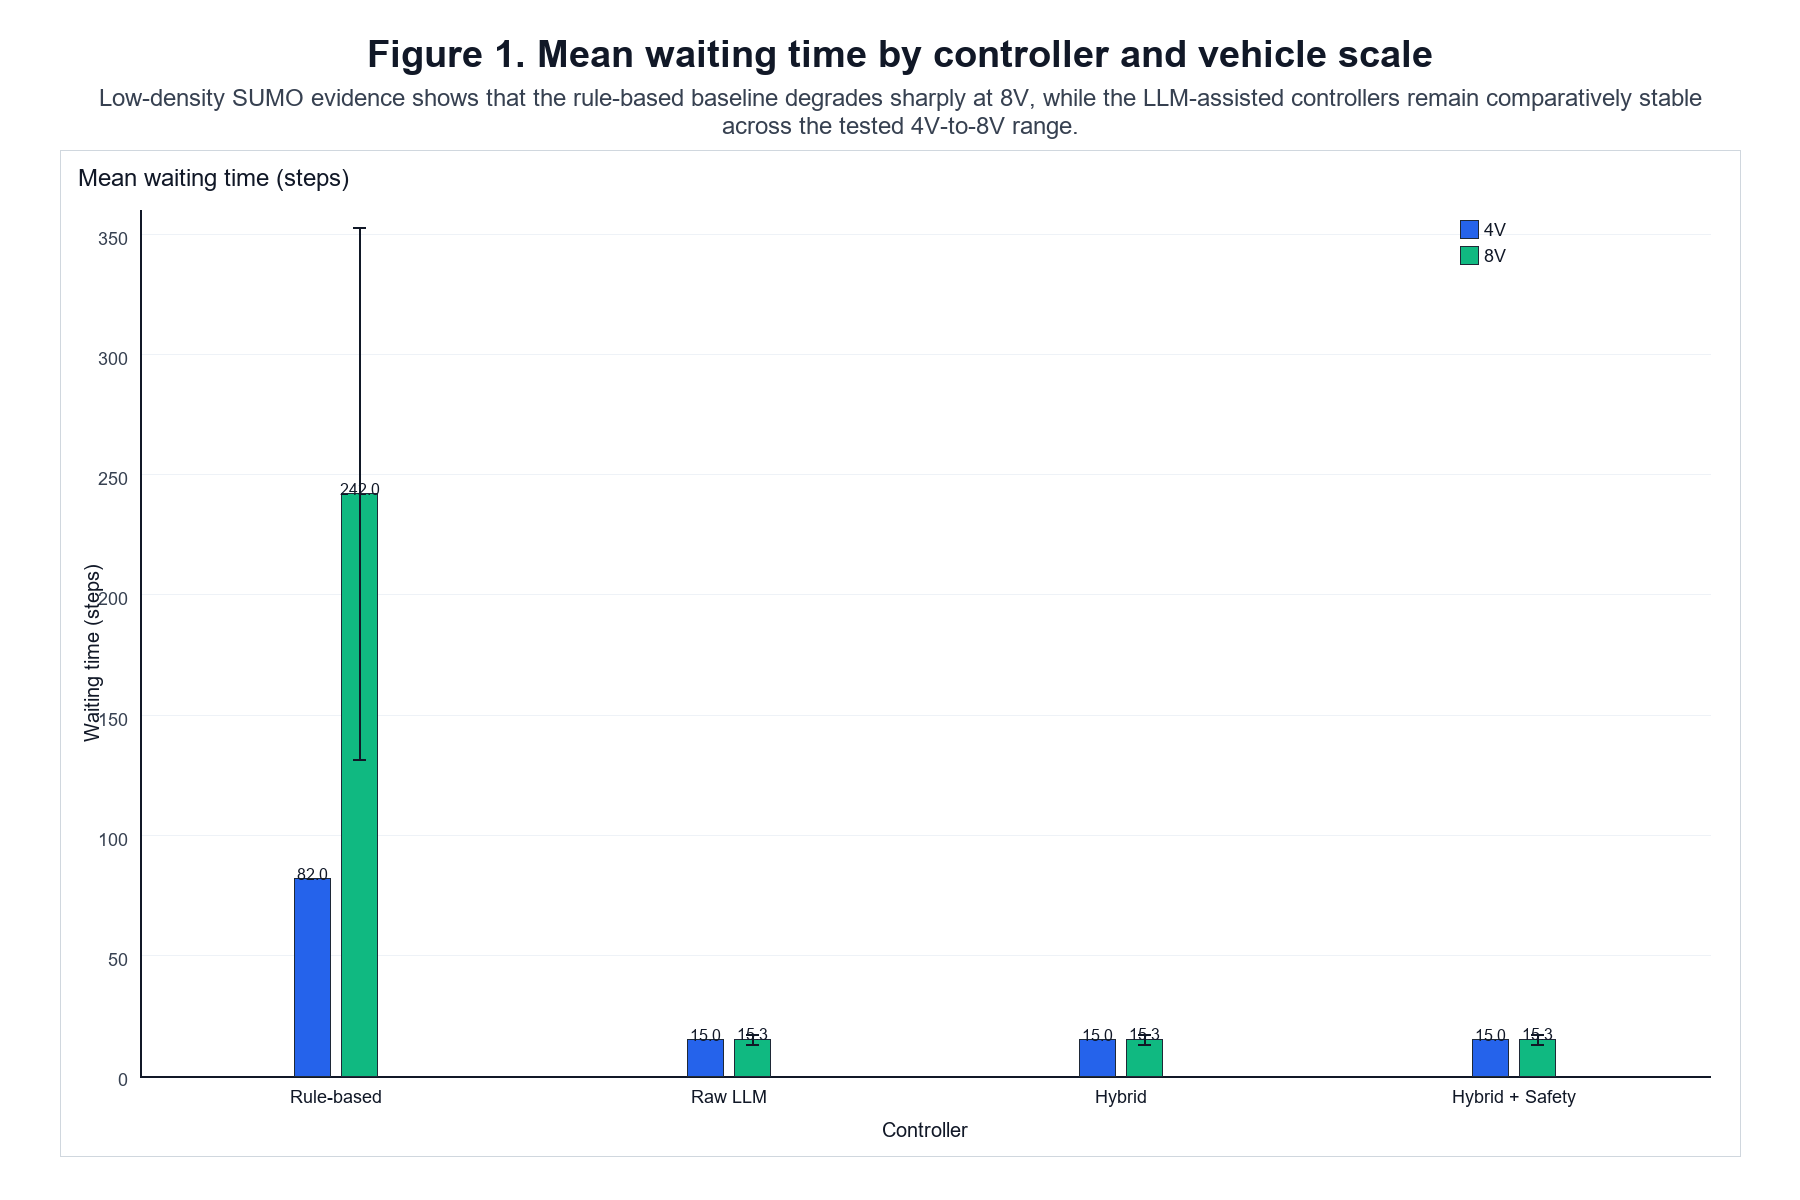
\includegraphics[width=0.75\textwidth]{figures/figure_1_mean_waiting_time.png}

\caption{Formal waiting figure for the retained 4V and 8V evidence boundary.}

\label{fig:waiting}

\end{figure*}



\begin{figure*}[t]

\centering

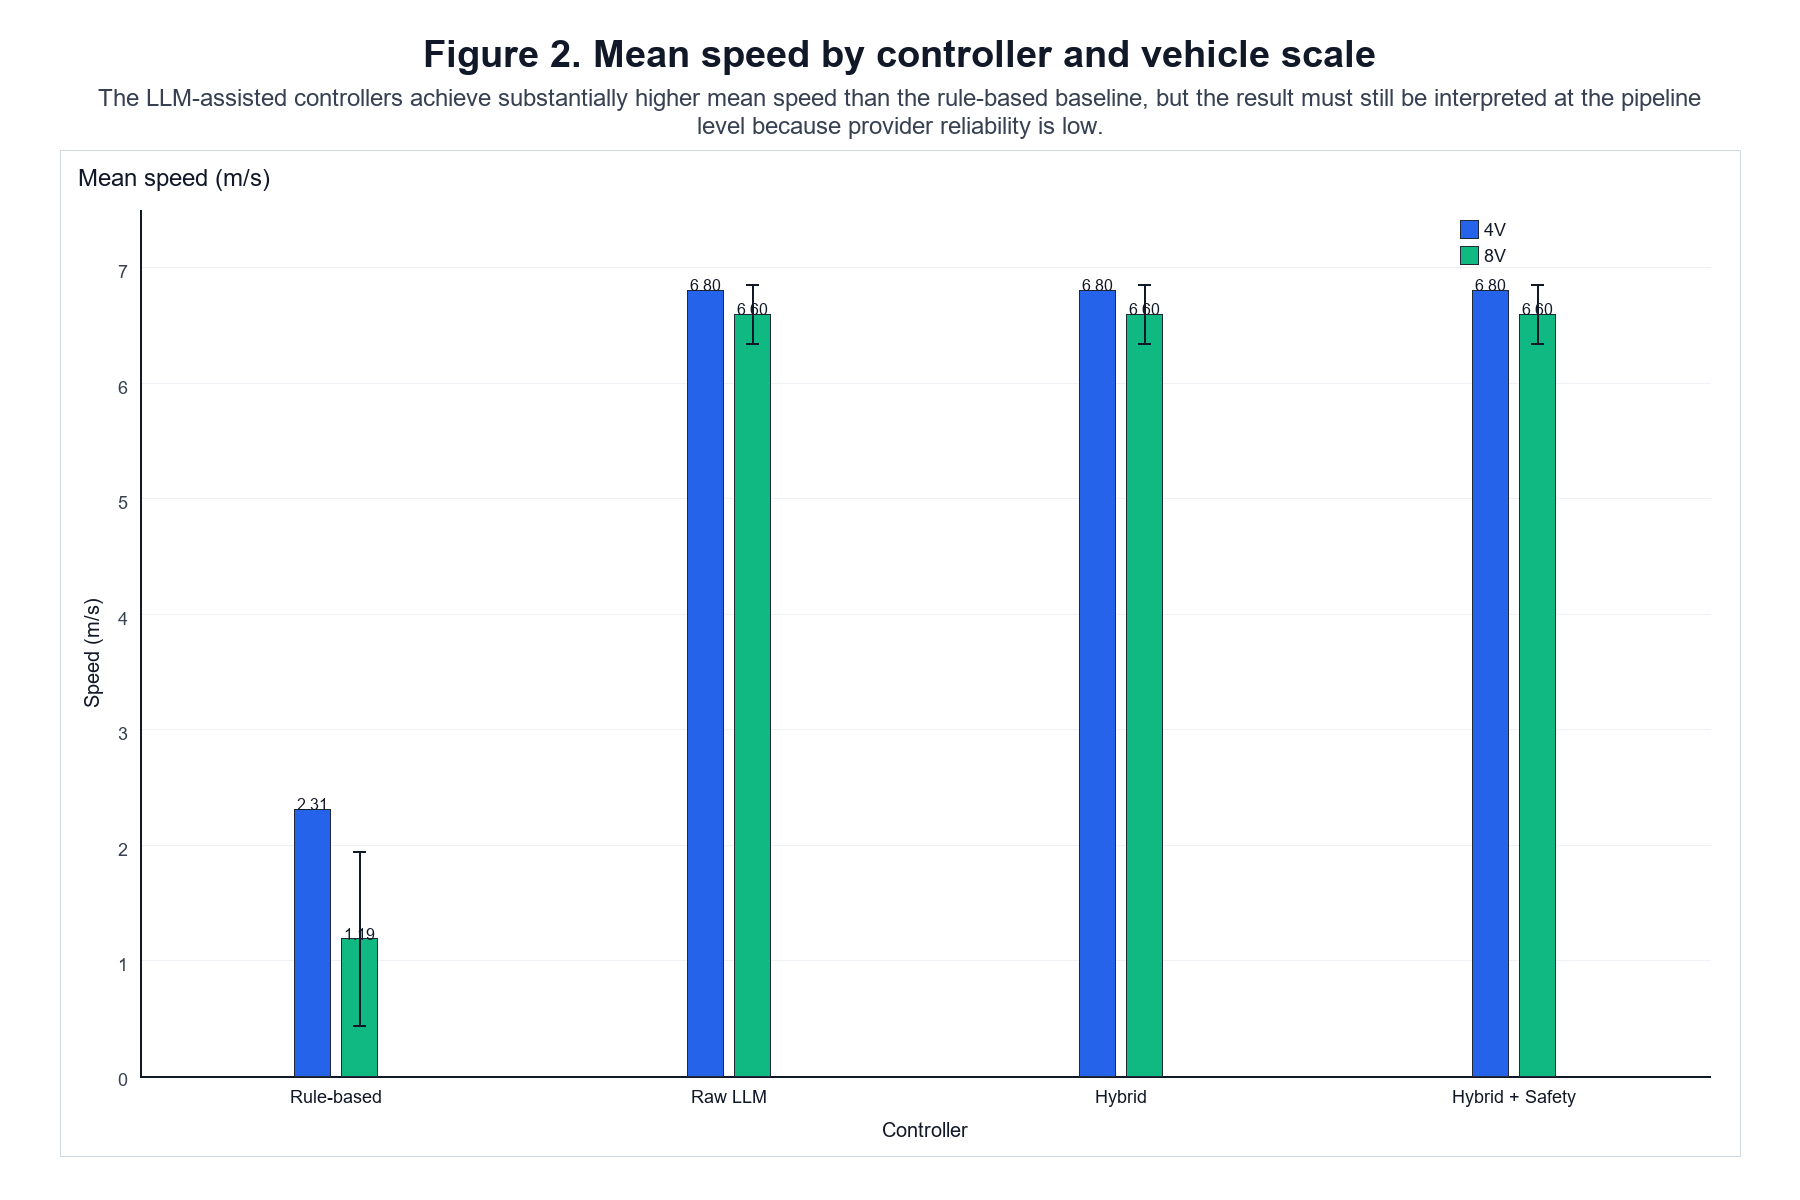
\includegraphics[width=0.75\textwidth]{figures/figure_2_mean_speed.png}

\caption{Formal mean-speed figure for the retained 4V and 8V evidence boundary.}

\label{fig:speed}

\end{figure*}



This result should not be interpreted as evidence of general scalability. The experiment considers only one intersection environment, two relatively small traffic scales, and three seeds per controller--scale condition. Higher-density traffic may introduce qualitatively different interactions, queue formation, or conflict patterns that are not represented by the current scenarios. The result supports robustness within the evaluated 4V--8V range rather than a claim that the controller will maintain the same performance as traffic density increases more generally.



\subsection{Provider Reliability and Fallback Dependence}



The traffic-level results show that the LLM-assisted pipelines operated efficiently, but provider diagnostics reveal a substantially different picture at the model-interaction level. As summarised in Table~\ref{tab:provider_reliability}, successful live-provider responses were rare during the retained formal experiments. For example, Raw LLM achieved a mean provider-success rate of approximately 6.29\% in the 4V condition and only 0.63\% in the 8V condition. The corresponding success rates for the Hybrid and Hybrid + Safety configurations were similarly low.



\begin{table*}[t]

\centering

\caption{Provider reliability and fallback behaviour in the formal evidence.}

\label{tab:provider_reliability}

\renewcommand{\arraystretch}{1.08}

\footnotesize

\begin{tabular}{p{1.55cm} p{0.82cm} p{1.65cm} p{1.65cm} p{1.65cm} p{1.5cm}}

\toprule

\textbf{Controller} & \textbf{Scale} & \textbf{Attempts} & \textbf{Successes} & \textbf{Success rate} & \textbf{Mean latency} \\

\midrule

Raw LLM & 4V & 53.000 $\pm$ 0.000 & 3.333 $\pm$ 4.714 & 6.29\% $\pm$ 8.89\% & 101.412 $\pm$ 29.695 ms \\

Raw LLM & 8V & 106.333 $\pm$ 0.471 & 0.667 $\pm$ 0.471 & 0.63\% $\pm$ 0.44\% & 76.846 $\pm$ 1.552 ms \\

Hybrid & 4V & 53.000 $\pm$ 0.000 & 3.000 $\pm$ 4.243 & 5.66\% $\pm$ 8.00\% & 111.021 $\pm$ 23.614 ms \\

Hybrid & 8V & 106.333 $\pm$ 0.471 & 0.333 $\pm$ 0.471 & 0.31\% $\pm$ 0.44\% & 79.035 $\pm$ 4.074 ms \\

Hybrid + Safety & 4V & 53.000 $\pm$ 0.000 & 3.000 $\pm$ 4.243 & 5.66\% $\pm$ 8.00\% & 96.152 $\pm$ 22.919 ms \\

Hybrid + Safety & 8V & 106.333 $\pm$ 0.471 & 0.333 $\pm$ 0.471 & 0.31\% $\pm$ 0.44\% & 76.398 $\pm$ 1.312 ms \\

\bottomrule

\end{tabular}

\end{table*}



\begin{figure*}[t]

\centering

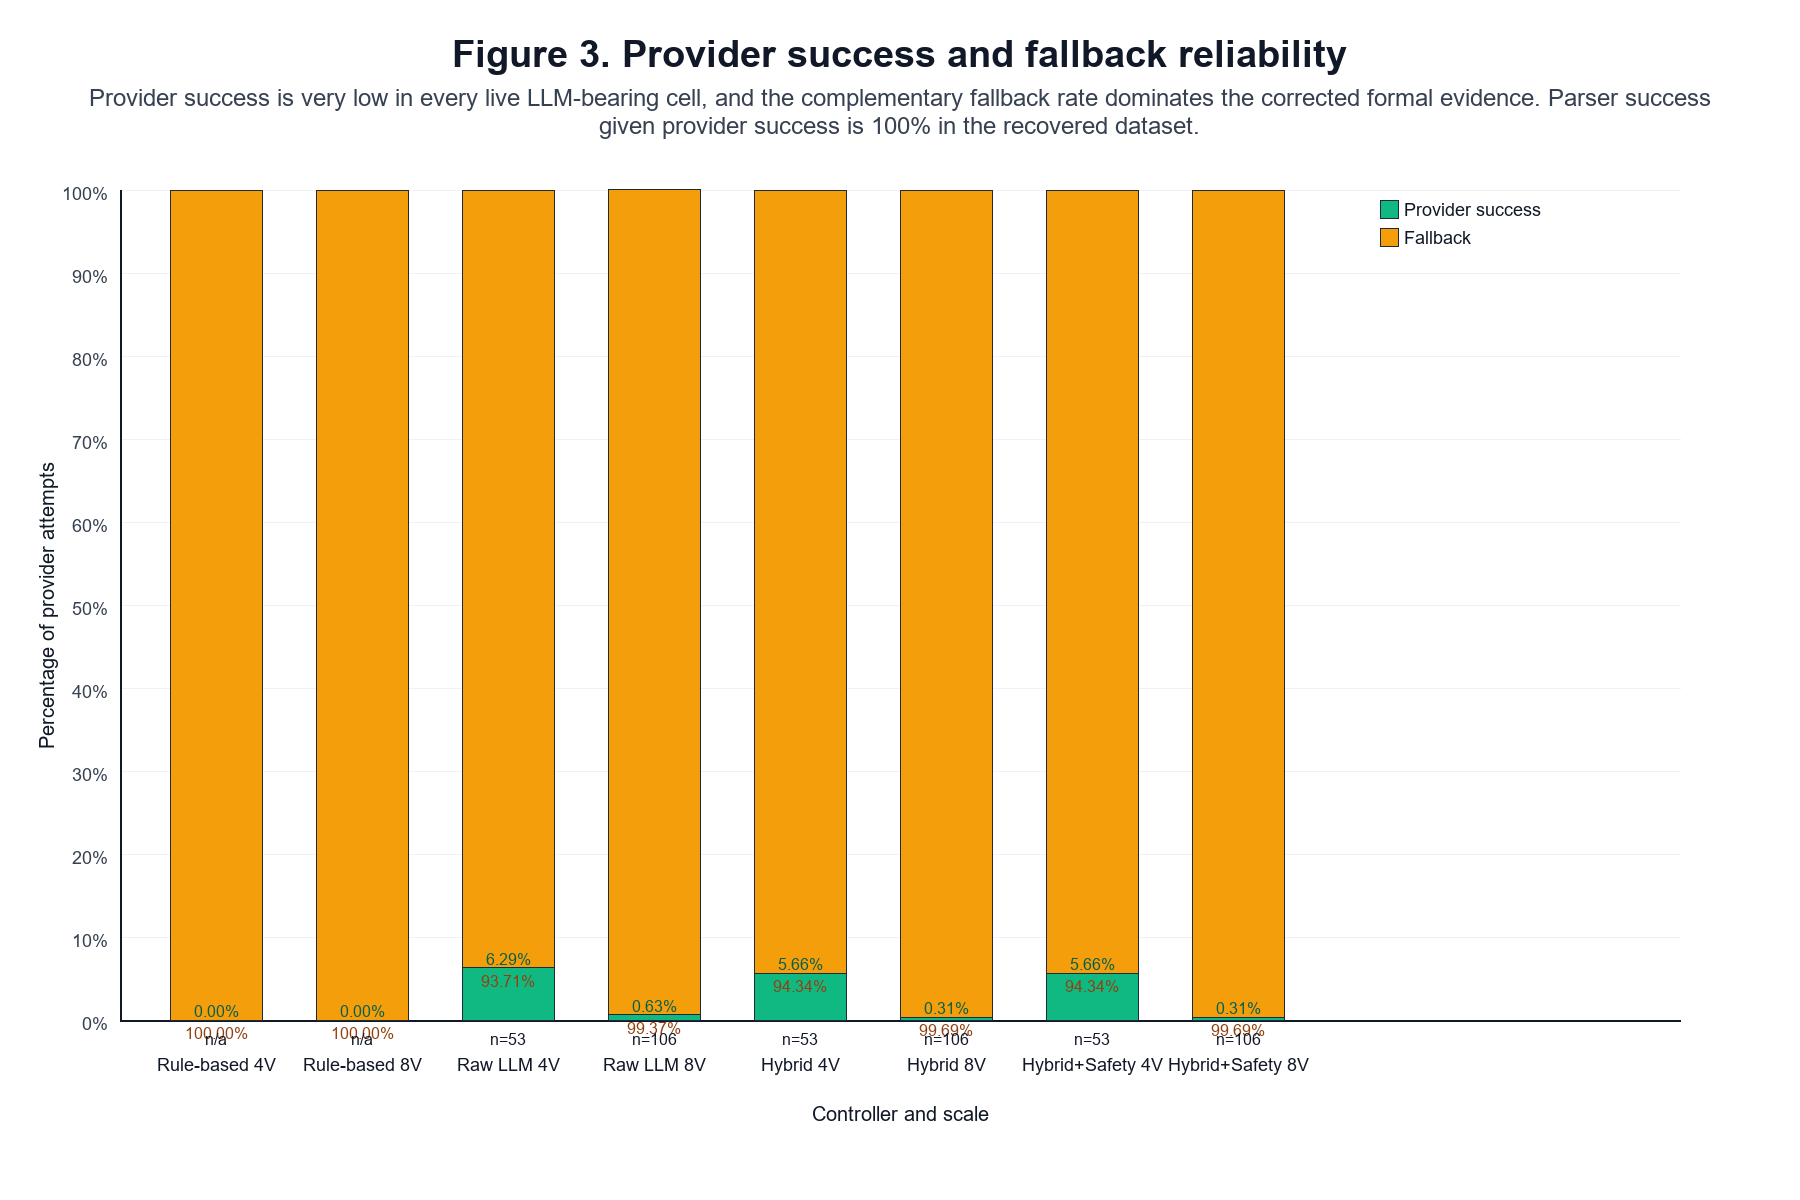
\includegraphics[width=0.48\textwidth]{figures/figure_3_provider_success_fallback.png}

\hfill

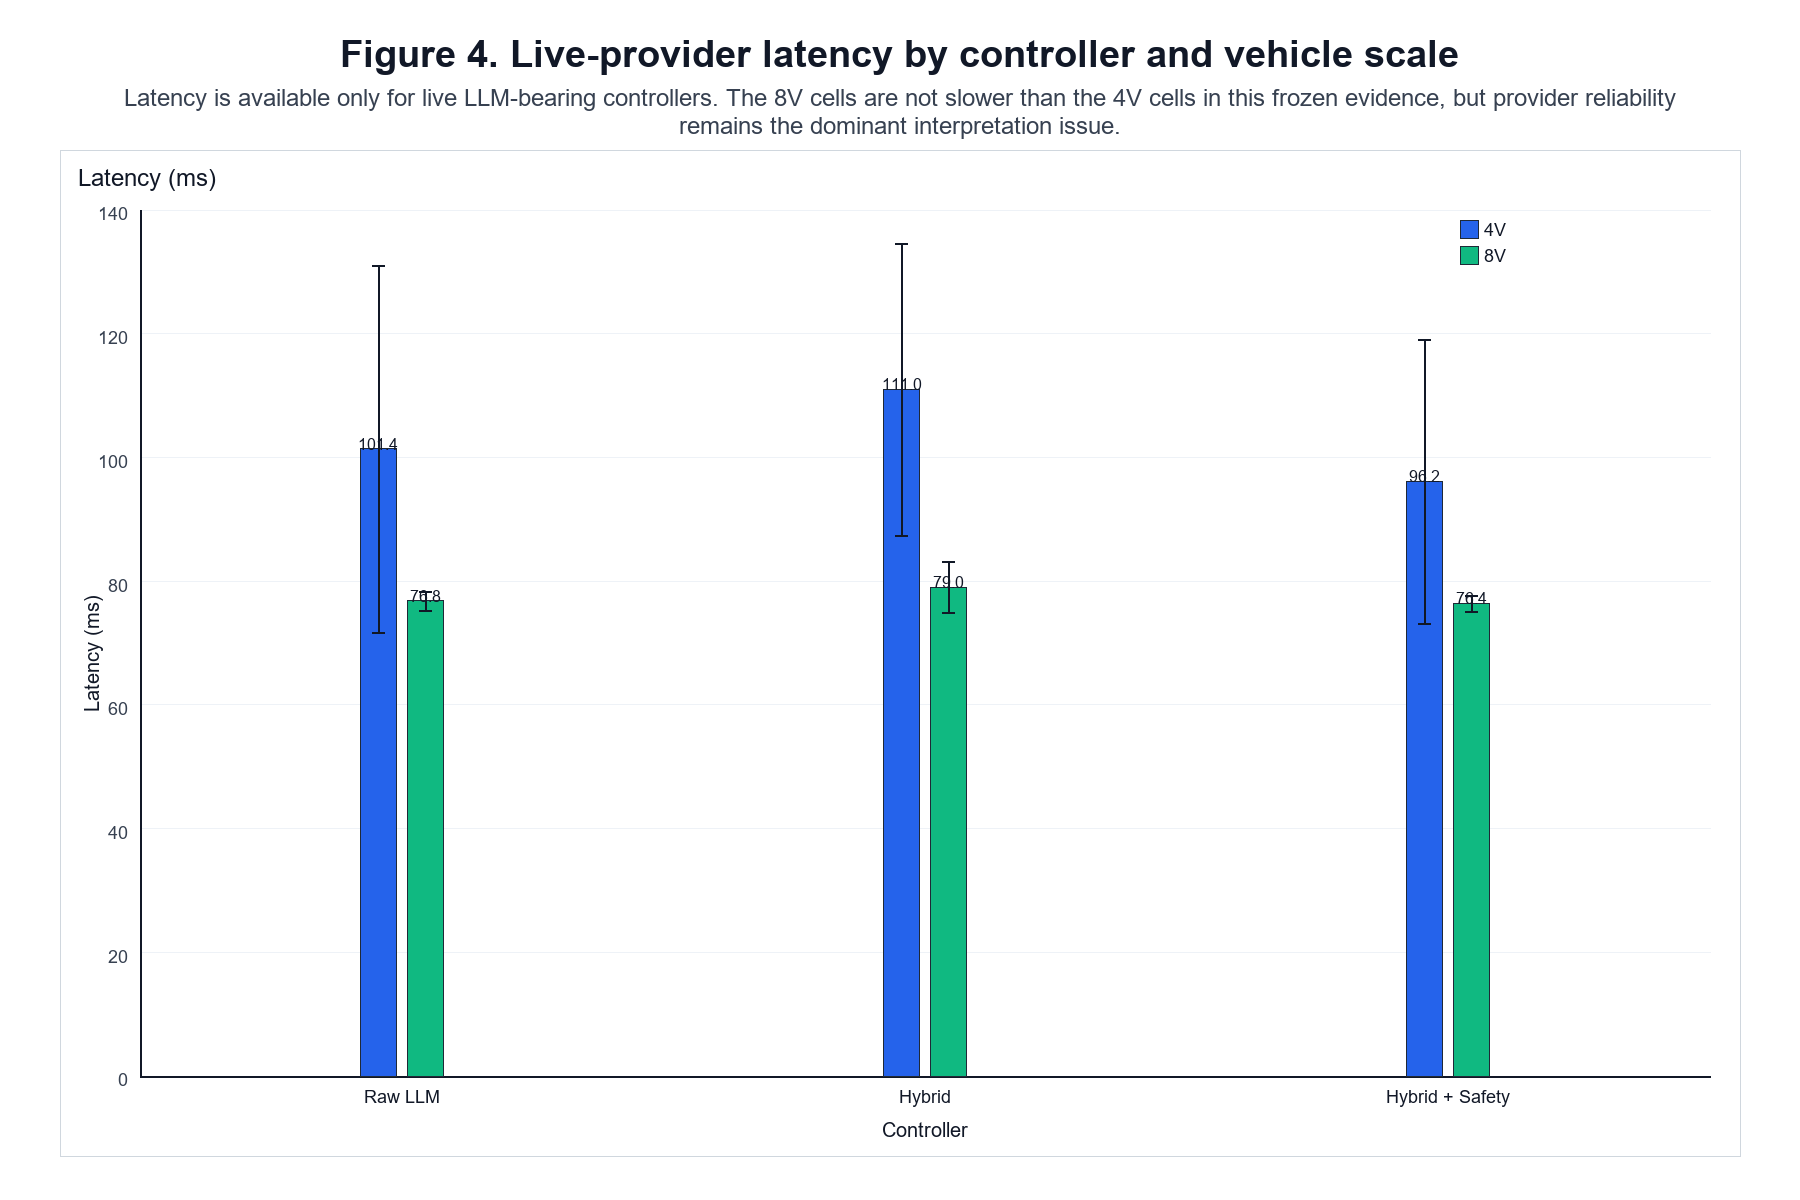
\includegraphics[width=0.48\textwidth]{figures/figure_4_latency.png}

\caption{Provider reliability and latency summaries for the formal live-provider runs. The left plot shows the strong fallback dominance, while the right plot shows the long-tail latency variation that accompanies the unreliable live-provider path.}

\label{fig:provider}

\end{figure*}



This creates an important discrepancy between system-level and provider-level performance. At the traffic level, the LLM-assisted pipelines achieved low operational waiting, high mean speed, full completion, and zero recorded collisions. At the provider level, however, the live model supplied usable responses for only a small proportion of logical requests. The majority of decision opportunities therefore could not have depended directly on successful live-model inference.



The deterministic fallback mechanism explains how these two observations can coexist. When a provider request failed or did not produce a usable decision, the pipeline could continue by substituting a deterministic action rather than terminating the simulation or forcing all affected vehicles to remain stopped. Consequently, provider failure did not necessarily translate into traffic failure. This behaviour is operationally desirable because it makes the controller robust to external-service failure, but it complicates interpretation of the traffic results.



Figure~\ref{fig:provider} illustrates the relationship between provider success and fallback use. Across the formal LLM-assisted runs, low provider success corresponds to substantial dependence on deterministic recovery. The formal experiment therefore demonstrates that the complete pipelines can remain operational under unreliable provider conditions, but it provides only limited evidence about the quality of successful LLM reasoning itself.



This observation changes the interpretation of the comparison reported in the previous subsection. The substantial difference between Rule-Based and the three LLM-assisted configurations cannot be interpreted simply as ``LLM versus rules''. The Rule-Based controller is one standalone deterministic policy, whereas the LLM-assisted pipelines contain a different deterministic fallback policy in addition to their model-facing components. When fallback supplies a large proportion of the effective control behaviour, the comparison becomes one between complete controller architectures rather than between language-model reasoning and deterministic reasoning in isolation.



The similarity between Raw LLM, Hybrid, and Hybrid + Safety further reinforces this attribution concern. Despite their different nominal architectures, their traffic-level results are effectively indistinguishable in the retained formal experiments. If the live provider rarely supplies usable decisions, there is correspondingly less opportunity for downstream LLM-dependent mechanisms to create observable divergence between the three configurations. The formal evidence therefore supports strong operational performance of the complete LLM-assisted pipelines, but it does not isolate an independent contribution from the live model.



Provider latency provides an additional practical constraint. Successful live requests introduce external inference delay that is absent from purely deterministic control. Latency is therefore relevant even when the returned decision is correct, because a traffic-control system must obtain decisions within an operationally useful time window. The recorded latency distribution shows that live inference is considerably more variable than deterministic decision logic. In the present simulator, this primarily affects experiment wall-clock execution rather than simulated vehicle dynamics, because the simulation waits for the decision pipeline. Nevertheless, the observation remains relevant to deployment: a real-time implementation would require explicit timing guarantees or asynchronous control mechanisms before external LLM inference could be treated as a dependable low-level control component.



Taken together, the formal provider diagnostics identify two distinct properties of the proposed architecture. First, deterministic recovery makes the overall pipeline resilient to provider failure. Second, that same resilience reduces the ability of aggregate traffic metrics to identify whether the LLM itself contributed to the observed outcome. The next analysis therefore examines the cooperative and safety stages before introducing a post-hoc experiment designed specifically to separate provider reliability from behavioural attribution.



\subsection{Cooperative Post-processing and Safety Verification}



The formal traffic results provide limited evidence for an independent contribution from the cooperative post-processing and safety-verification stages. Raw LLM, Hybrid, and Hybrid + Safety produced essentially identical operational waiting and mean-speed results at both evaluated traffic scales. Completion was also 100\% and no collisions were recorded for any of the three configurations. At the aggregate traffic level, the additional deterministic stages therefore did not produce measurable separation under the retained scenarios.



This result should not be interpreted as evidence that cooperative processing or safety verification is inherently ineffective. Demonstrating an independent contribution requires the corresponding mechanism to be activated under conditions in which its intervention can alter an otherwise different decision. If candidate actions are already compatible, a cooperative postprocessor may legitimately preserve them. Similarly, if no candidate action violates the implemented safety conditions, a safety verifier can remain inactive while the scenario still completes without collision.



The zero-collision result is particularly important to interpret conservatively. Because all controller configurations recorded zero collisions, collision count is saturated in the present experiment and cannot discriminate between the safety mechanisms. It would therefore be inappropriate to attribute collision-free operation specifically to the Hybrid + Safety architecture. Evidence for such a claim would require scenarios that generate safety-relevant candidate decisions and sufficient verifier interventions to compare outcomes with and without the additional stage.



The similarity between the three LLM-assisted configurations also interacts with the provider-reliability limitation described above. When live-model success is low and deterministic fallback supplies much of the effective control behaviour, the opportunity for model-dependent downstream stages to generate distinct trajectories is reduced. The formal experiment can therefore establish the behaviour of the complete pipelines, but it cannot reliably isolate the incremental effects of cooperative post-processing or safety verification.



These observations motivate two separate conclusions. First, the additional stages remain technically meaningful parts of the modular architecture because they provide explicit locations for cooperative intervention and deterministic verification. Second, the retained scenarios do not provide sufficient behavioural activation to demonstrate their independent performance benefit. More discriminative scenarios and component-level ablations are required before stronger claims can be made.



\subsection{Post-hoc Gemini Attribution Analysis}



The formal experiment identifies a central attribution problem: the LLM-assisted pipelines achieve strong traffic performance while successful live-provider responses are rare. Under these conditions, it is not possible to determine from aggregate traffic metrics whether a reliable LLM would behave differently from the deterministic fallback. A supplementary post-hoc analysis was therefore conducted to remove provider failure as the dominant confounding factor.



This analysis used the Raw LLM 4V seed-1 scenario with a subsequently validated Gemini configuration. The diagnostic is deliberately kept outside the 24-run formal experimental matrix because it was introduced after inspection of the formal provider evidence and was executed under different provider conditions. Its purpose is not to strengthen the formal controller comparison through additional samples, but to investigate the source of the behaviour observed in the LLM-assisted pipeline.



In the reliable Gemini run, all 53 logical provider requests completed successfully and all 53 responses were parsed successfully. No deterministic fallback was triggered. The scenario also completed normally, with all four vehicles arriving and no recorded collision. This removes the dominant reliability problem observed in the formal runs and provides a cleaner opportunity to observe the decisions produced by the live model.





\begin{table}[t]

\centering

\caption{Post-hoc attribution evidence for the reliable Gemini 4V seed1 diagnostic.}

\label{tab:posthoc_attribution}

\renewcommand{\arraystretch}{1.08}

\footnotesize

\begin{tabular}{p{1.9cm} p{1.55cm} p{1.1cm} p{1.2cm} p{1.9cm}}

\toprule

\textbf{Condition} & \textbf{Provider path} & \textbf{Waiting} & \textbf{Mean speed} & \textbf{Decision agreement} \\

\midrule

Reliable Gemini 4V seed1 & 53/53 success, 0 fallback & 11.0 & 7.58 m/s & 132/132 raw and final \\

Fallback-only 4V seed1 & deterministic fallback only & 11.0 & 7.58 m/s & matched action stream \\

High-discrimination subset & same diagnostic slice & -- & -- & 39/39 raw and final \\

\bottomrule

\end{tabular}

\end{table}





However, eliminating provider failure did not produce an additional traffic-performance difference. As shown in Table~\ref{tab:posthoc_attribution}, the reliable Gemini run produced an operational waiting value of 11.0 steps and a mean speed of 7.58~m/s. A fallback-only ablation under the corresponding comparison produced the same values. The reliable-model condition therefore did not improve the measured traffic outcome beyond the deterministic fallback in this scenario.



Traffic-level equality alone could still conceal different internal decisions that happen to produce similar aggregate metrics. The analysis therefore compared aligned vehicle-level decisions. Across 132 comparable decision records, the Gemini raw decisions agreed with the fallback decisions on all 132 rows. The final executed decisions also agreed on all 132 rows. Thus, the absence of a traffic-level difference was accompanied by complete decision-level agreement rather than by different decisions being subsequently mapped to the same aggregate outcome.



A further analysis focused on states expected to provide greater opportunity for behavioural differentiation. Eleven mixed route-group states were identified from simulation steps 14--24, containing 39 comparable vehicle-level decisions. These states included simultaneous control of multiple vehicles and therefore represented more discriminative interaction conditions than isolated single-vehicle decisions. Nevertheless, Gemini and the deterministic fallback again agreed on all 39 raw decisions and all 39 final decisions.



This evidence rules out one important explanation for the earlier formal result. The lack of observable LLM-specific benefit cannot be attributed solely to provider failure: once provider success reached 53/53 with zero fallback, the live model still reproduced the deterministic policy on every aligned decision examined. The attribution problem therefore changes from one of \emph{provider reliability} to one of \emph{behavioural identifiability}.



The result also indicates that downstream deterministic processing was not responsible for erasing an initially different model policy in this diagnostic. Gemini and fallback already agreed at the raw-decision level before comparison of the final executed actions. The observed equivalence therefore originates upstream of the final decision stage rather than being created solely by cooperative or safety post-processing.



One plausible explanation is the semantic overlap between the model prompt and the deterministic fallback policy. Both mechanisms encode similar priorities concerning movement compatibility, progress, and conflict avoidance. A sufficiently constrained LLM can therefore produce valid and reliable responses while still implementing behaviour that is functionally indistinguishable from the deterministic policy used as its substitute. Under such conditions, increasing provider reliability improves confidence that the model is actually being executed, but does not by itself create the behavioural variation required to identify an independent model contribution.



The post-hoc result should therefore not be interpreted as evidence that LLM reasoning is generally incapable of contributing to intersection control. It demonstrates a narrower limitation of the current method: within the tested 4V state distribution and the frozen prompt/fallback semantics, the reliable model does not exhibit observable behavioural divergence from deterministic fallback. Establishing an independent LLM effect would require an experimental design in which the model and deterministic comparator have meaningful opportunities to select different valid actions.



\section{Discussion and Limitations}



\subsection{Interpretation of the Main Findings}



The results reveal an important separation between the performance of the complete control pipeline and the contribution that can be attributed specifically to the live language model. At the system level, the outcome is clear: all three LLM-assisted controller configurations substantially outperform the selected Rule-Based baseline in operational waiting and mean speed across the retained 4V and 8V scenarios, while maintaining full completion and zero recorded collisions. If evaluation were restricted to conventional traffic metrics, this would appear to provide strong evidence in favour of the LLM-assisted approach.



The internal diagnostics, however, change the interpretation of this result. Provider success during the formal experiments was low, meaning that a large proportion of the effective control behaviour was supplied through deterministic mechanisms rather than successful live-model inference. The formal experiment therefore demonstrates that the proposed \emph{pipeline architecture} performs well relative to the selected Rule-Based baseline, but it does not demonstrate that successful LLM reasoning independently causes this improvement.



This distinction is not merely terminological. The deterministic fallback is itself a functional traffic-control policy and differs from the standalone Rule-Based baseline. Consequently, comparing Rule-Based with Raw LLM does not reduce to a clean comparison between deterministic control and LLM control when the model-facing pipeline frequently activates fallback. Strong Raw LLM traffic performance under these conditions can be evidence of a robust architecture while simultaneously providing weak evidence for an independent model contribution.



The post-hoc Gemini analysis strengthens this interpretation by removing provider failure as the dominant confounding factor. With 53/53 successful logical requests and no fallback activation, the live model was demonstrably participating in the decision process. Nevertheless, its traffic outcome remained identical to the fallback-only comparison, and its decisions agreed with fallback on all 132 aligned vehicle-level records. Complete agreement also remained in the 39 decisions selected from higher-discrimination mixed route-group states. The absence of an observable LLM-specific effect therefore persists even after reliable model execution is established.



Taken together, the formal and post-hoc evidence supports a two-part conclusion. First, the modular LLM-assisted pipelines provide a strong system-level result under the evaluated scenarios. Second, the current experiment provides limited evidence that the LLM itself contributes behaviour beyond the deterministic policy already embedded in the pipeline. These conclusions are compatible rather than contradictory because system robustness and model-specific effectiveness are different properties.



\subsection{Answers to the Research Questions}



\textbf{RQ1: How does the Raw LLM pipeline compare with a standalone rule-based controller in traffic efficiency and completion?}



At the complete-pipeline level, Raw LLM performs substantially better than the selected Rule-Based baseline in the evaluated scenarios. It produces lower operational waiting and higher mean speed in both 4V and 8V conditions while retaining 100\% completion and zero recorded collisions. RQ1 can therefore be answered positively at the pipeline level.



This result should not, however, be interpreted as evidence that live LLM reasoning independently outperforms rule-based reasoning. The formal Raw LLM configuration contains deterministic fallback and interface logic, and provider diagnostics show that successful model responses were uncommon during the formal experiment. The appropriate conclusion is therefore that the \emph{Raw LLM pipeline} outperformed the selected Rule-Based controller, not that the LLM model itself did so.



\textbf{RQ2: Does cooperative post-processing provide an observable benefit beyond Raw LLM control?}



No independent benefit is observed under the retained experimental conditions. Hybrid and Raw LLM produce essentially the same aggregate traffic outcomes. The available evidence therefore does not demonstrate that cooperative post-processing improves traffic performance beyond the Raw LLM pipeline in these scenarios.



This is an absence of discriminative evidence rather than evidence that cooperative processing is generally ineffective. A cooperative mechanism can only demonstrate an incremental contribution when the evaluated state distribution creates candidate decisions that require meaningful modification. More targeted conflict scenarios would be required to establish whether the postprocessor provides a measurable advantage when its intervention conditions are activated.



\textbf{RQ3: Does deterministic safety verification provide an observable benefit beyond the Hybrid controller?}



The retained experiment does not identify an independent safety-verification benefit. Hybrid and Hybrid + Safety both achieve full completion and zero collisions, and their aggregate traffic outcomes are effectively indistinguishable. Because collision count is already zero without the additional verifier, the primary safety metric is saturated and cannot establish that the safety stage caused the collision-free result.



The appropriate answer to RQ3 is therefore that no incremental effect was observed under the tested conditions. Stronger evaluation would require deliberately discriminative but valid interaction scenarios in which unsafe or conflicting candidate decisions are sufficiently likely to activate the verifier.



\textbf{RQ4: How do the evaluated controller pipelines behave when the tested traffic scale increases from 4V to 8V?}



The Rule-Based controller deteriorates substantially as the tested scale increases: operational waiting rises and mean speed falls. In contrast, the three LLM-assisted pipelines retain approximately the same waiting and speed levels across the 4V and 8V scenarios while maintaining full completion and zero collisions. The retained evidence therefore indicates greater robustness of the complete LLM-assisted pipelines within the evaluated 4V--8V range.



This result is not evidence of general scalability. Only two relatively small traffic scales, one intersection setting, and three seeds per condition are evaluated. RQ4 therefore supports robustness to the specific increase examined in this study rather than unrestricted scalability to dense or realistic traffic networks.



\subsection{Traceability and Causal Identifiability}



A central methodological finding of this study is that decision traceability and causal identifiability are related but distinct properties. The implemented provenance system can reconstruct whether a provider request occurred, whether it succeeded, whether parsing succeeded, whether fallback was activated, and how a candidate decision changed before execution. This information is essential for interpreting an LLM-assisted controller because traffic outcomes alone cannot reveal which internal component produced the executed behaviour.



However, complete traceability does not guarantee that the independent effect of a component can be identified. Causal attribution requires meaningful behavioural variation between the mechanisms being compared. If a live model and deterministic fallback consistently select the same action for the same state, provenance can confirm that the model generated the action but cannot demonstrate that using the model changed the resulting traffic behaviour.



The post-hoc Gemini experiment illustrates this distinction. Once request provenance was available and provider reliability reached 100\%, the origin of the model decisions became clearly traceable. Nevertheless, Gemini and fallback agreed on every aligned raw decision examined. There is therefore no counterfactual separation between the two policies in the observed state distribution: replacing the successful model output with fallback would not have changed any of the compared actions.



This result identifies behavioural identifiability as a limitation distinct from provider reliability. Provider reliability asks whether the model can be executed consistently. Behavioural identifiability asks whether the model produces decisions sufficiently different from the deterministic comparator for its contribution to be measured. The former was addressed by the reliable Gemini configuration, while the latter remained unresolved.



The likely source of this limitation is the substantial semantic overlap between the frozen LLM instructions and the deterministic fallback policy. Both mechanisms encode similar preferences concerning progress, movement compatibility, and conflict avoidance. Such overlap is operationally reasonable because fallback is intended to provide safe and coherent behaviour when model inference is unavailable. Experimentally, however, it reduces the probability that the two mechanisms will disagree. A robust fallback can therefore simultaneously improve system reliability and weaken the identifiability of the LLM's independent contribution.



This creates a general design tension for hybrid LLM systems. Deterministic components are desirable for reliability and safety, but the stronger and more behaviourally similar these components become, the more difficult it is to determine whether the probabilistic component provides additional value. Evaluation should therefore consider not only whether fallback exists, but also whether the experimental state distribution contains situations in which the model and fallback can reasonably produce different valid decisions.



\subsection{Relation to Existing Literature}



The pipeline-level results are consistent with the broader motivation for cooperative intersection management. Previous work on autonomous intersection control has shown that coordinating access to a shared conflict region can reduce unnecessary waiting compared with conservative or fixed control strategies \cite{Dresner2008,Safarov2022,Zhao2025}. The present results similarly show that the evaluated LLM-assisted pipelines maintain substantially lower waiting than the selected Rule-Based baseline as the tested scale increases from 4V to 8V.



At the same time, the attribution analysis qualifies how LLM-related results should be interpreted. Existing work has demonstrated the potential of language models for planning, embodied reasoning, and autonomous-driving decision support \cite{Huang2022,Driess2023,Wen2023,Jin2023,Cui2024}. These studies motivate the use of LLMs as high-level reasoning components, but the present experiment highlights an additional evaluation requirement when such models are embedded within hybrid systems: the performance of the complete architecture should not automatically be attributed to the model.



This observation is particularly relevant to architectures that combine probabilistic reasoning with deterministic safeguards. Such designs are attractive because they preserve operational behaviour when model inference fails, but they introduce alternative causal pathways from input state to executed action. Provider success, parser success, fallback activation, downstream intervention, and final traffic outcome therefore represent different levels of evidence.



The findings consequently complement existing LLM-for-autonomy research by emphasising evaluation rather than proposing a new claim of model superiority. A model may be reliable, structured, and successfully integrated while still failing to demonstrate behaviour beyond a deterministic comparator. Conversely, an unreliable model can be embedded in a pipeline that performs well because deterministic mechanisms preserve operation. Evaluating both situations requires component-level evidence in addition to aggregate task performance.



\subsection{Limitations}



Several limitations constrain the generality and causal strength of the reported findings.



First, the simulation study uses a single unsignalised-intersection environment and only two traffic scales. Although the increase from 4V to 8V creates a clear difference in the behaviour of the Rule-Based baseline, it does not represent the diversity of traffic demand, intersection geometry, route distribution, or interaction patterns that would occur in realistic deployment. The results should therefore be interpreted as evidence for the evaluated scenarios rather than general autonomous-intersection performance.



Second, only three seeds are retained for each controller--scale condition. This provides some indication of run-to-run variability but is insufficient for strong inferential statistical analysis. The reported means, standard deviations, percentage changes, and comparisons are consequently descriptive.



Third, the primary delay measure is operational waiting derived from the implemented simulation trace rather than a comprehensive queueing-delay metric. It is useful for consistent comparison within the experiment, but it should not be interpreted as equivalent to every conventional traffic-engineering definition of delay.



Fourth, the safety evaluation is limited by the absence of recorded collisions across the retained formal runs. Zero collisions are desirable operationally but provide little discriminative information when all controllers achieve the same outcome. The current experiment therefore cannot establish an independent safety benefit from the deterministic verifier. More challenging conflict-oriented scenarios would be required to evaluate that mechanism directly.



Fifth, live-provider reliability during the formal experiment was poor. Deterministic fallback allowed the LLM-assisted pipelines to complete despite these failures, but the resulting traffic performance cannot be interpreted as a clean measurement of live-model behaviour. The later Gemini diagnostic addresses this limitation only partially because it is a supplementary post-hoc experiment rather than part of the original 24-run formal matrix.



Sixth, the reliable Gemini analysis is restricted to the 4V seed-1 condition. Although it provides strong decision-level evidence within that scenario, it does not establish that Gemini and fallback would remain behaviourally identical across other seeds, larger traffic scales, different prompts, or more complex conflict distributions.



Finally, the frozen prompt and deterministic fallback encode substantially overlapping control semantics. This is the most important limitation for model-level attribution. The experiment can establish that the two mechanisms behave similarly in the observed states, but it cannot determine whether an LLM would provide additional value in situations requiring reasoning not already captured by the deterministic policy.



\subsection{Implications for Future Experimental Design}



Future work should therefore prioritise discriminative experimental design rather than simply increasing the number of identical runs. Additional seeds and traffic scales would improve statistical coverage, but they would not solve the attribution problem if the LLM and fallback continue to produce the same actions.



A stronger evaluation should construct or systematically identify states in which multiple actions remain operationally plausible and in which the deterministic comparator has a known limitation. Examples could include asymmetric arrival patterns, competing route groups, larger simultaneous vehicle sets, or interaction states in which local deterministic priorities create unnecessary conservatism. The objective would not be to construct artificially favourable cases for the LLM, but to create situations in which different reasoning mechanisms have a genuine opportunity to produce distinguishable behaviour.



Future experiments should also include explicit component ablations. A reliable live-model condition should be compared with fallback-only control using the same state distribution, while cooperative and safety stages should be enabled and disabled independently. Decision disagreement, intervention frequency, and resulting traffic changes can then be measured together. This would provide a stronger basis for separating model contribution, fallback contribution, cooperative intervention, and safety intervention.



Provider reliability should additionally be treated as an experimental variable rather than merely an implementation detail. Stable structured output, bounded latency, request provenance, and explicit failure classification are prerequisites for meaningful model evaluation. Where real-time operation is considered, asynchronous inference or bounded-time decision architectures may also be required because the latency of remote LLM inference is substantially more variable than deterministic control.



Finally, future evaluation should preserve the attribution-aware evidence structure developed in this work. Traffic performance should remain the primary measure of system usefulness, but model-specific claims should require corresponding provider reliability, provenance, ablation, and behavioural divergence evidence. This would make it possible to distinguish systems that merely contain an LLM from systems in which the LLM demonstrably changes the resulting control behaviour.



\section{Conclusion}



This study developed and evaluated a modular LLM-assisted control pipeline for cooperative decision making at an unsignalised intersection in SUMO. The architecture separates structured state representation, live-provider inference, parsing and validation, deterministic fallback, cooperative post-processing, safety verification, execution, and decision provenance. This separation was designed not only to improve operational robustness, but also to make the contribution of individual pipeline stages observable during evaluation.



The formal experiment retained 24 valid runs across four controller configurations, two traffic scales, and three random seeds. At the complete-pipeline level, Raw LLM, Hybrid, and Hybrid + Safety achieved substantially lower operational waiting and higher mean speed than the selected Rule-Based baseline while maintaining 100\% completion and zero recorded collisions. The Rule-Based controller also degraded more strongly when the tested scale increased from 4V to 8V, whereas the three LLM-assisted pipelines remained comparatively stable within the evaluated range.



However, provider diagnostics substantially limit the interpretation of this traffic-level advantage. Successful live-model responses were rare during the formal experiment, meaning that deterministic fallback supplied much of the effective behaviour of the LLM-assisted pipelines. The formal results therefore support a pipeline-level performance advantage, but they do not establish that successful LLM reasoning independently caused that advantage.



A supplementary post-hoc Gemini diagnostic was used to investigate this attribution problem under reliable provider operation. All 53 logical provider requests succeeded, parser success was complete, and no fallback was triggered. Despite this, the reliable Gemini condition produced the same measured traffic performance as fallback-only control and agreed with fallback on all 132 comparable vehicle-level decisions. Complete agreement was also retained across 39 decisions selected from higher-discrimination mixed route-group states. The lack of an observable LLM-specific effect therefore cannot be explained only by provider failure or by downstream deterministic stages overwriting different model decisions.



The strongest contribution of this work is consequently methodological. The study demonstrates that successful system-level performance, provider reliability, traceability, and model-level causal contribution are distinct evaluation questions. A pipeline can remain operational under provider failure because of deterministic recovery, and a fully traceable model can still be behaviourally indistinguishable from fallback. Future LLM-assisted control experiments should therefore combine traffic metrics with provider diagnostics, provenance, component ablation, and deliberately discriminative scenarios before attributing system-level improvements to the model itself.



Within the scope of the present study, the evidence supports the effectiveness and reproducibility of the complete fallback-capable control pipeline relative to the selected Rule-Based baseline. It does not support independent LLM superiority, a standalone cooperative-postprocessing benefit, an independent safety-verification benefit, or general scalability beyond the tested 4V--8V setting.



\bibliographystyle{IEEEtran}

\bibliography{References}



\end{document}
